\documentclass[11pt]{article}

\usepackage[latin1]{inputenc}
\usepackage[a4paper,top=1in,left=1in,right=1in,bottom=1in]{geometry}
\usepackage[pdftex]{graphicx}
\usepackage{natbib}

\begin{document}

\pagestyle{empty}

\centerline{

\includegraphics[height=22mm]{Logos/logo_uga.png}
\hspace{5mm}

\includegraphics[height=22mm]{Logos/logo_cnrs.png}
\hfill

\includegraphics[height=22mm]{Logos/logo_ige.png}
}

\vspace{20mm}

\begin{center}

{\Huge\bf EnsAnam}

\vspace{10mm}
{\Large\bf Ensemble Anamorphosis Transformation}

\vspace{10mm}
{\Large\bf User's guide}

\vspace{10mm}
{\large\bf Jean-Michel Brankart}

\vspace{5mm}
{\tt http://pp.ige-grenoble.fr/pageperso/brankarj/}

\vspace{5mm}
{\large Institut des G\'eosciences de l'Environnement}

\vspace{1mm}
{\large Universit\'e Grenoble Alpes, CNRS, France}

\end{center}

\vspace{20mm}
The purpose of EnsAnam is to provide tools
to apply anamorphosis transformation to ensemble simulations.
The objective is to transform the marginal distribution of all variables
to the same distribution defined by the user
(usually a normalized Gaussian distribution).

The tools are provided as a library of modules,
which can be easily plugged in any existing software.
This library includes:

\begin{itemize}
\item the computation of quantiles of the input ensemble (defining the transformation),
\item the application of the transformation to any state vector,
\item the transformation of observations.
\end{itemize}

\clearpage

\pagestyle{plain}

\section{Description of the method}

The purpose of anamorphosis transformation is
to apply a nonlinear transformation to the simulated variables,
so that all marginal distributions become identical
(usually a normalized Gaussian distribution).
This is done by computing the transformation~$A_i$
associated to each variable~$x_i$ of the vector~${\bf x}$,
so that $z_i=A_i(x_i)$ has the required marginal distribution,
usually ${\cal N}(0,1)$.
By combining these univariate transformations,
we can write the transformed vector: ${\bf z} = A({\bf x})$.

Our basic assumptions to compute the transformation~$A$
are that: (i)~the probability distribution of~${\bf x}$
is described by an ensemble of moderate size,
so that the transformation~$A$ can only be approximately identified, and
(ii)~the size of the vector~${\bf x}$ can be very large
so that the practical algorithm (to compute and apply $A$ and~$A^{-1}$)
must contain as few operations as possible.

Potential applications of this method are numerous,
but the target application for which these modules have been developed
is the transformation of the ensemble observational update
so that the prior marginal distributions become Gaussian.
The ensemble observational update is based on the Bayes theorem:

\begin{equation}
p^a({\bf x}) = p({\bf x}|{\bf y}^o) = p^f({\bf x}) \;\; p \left[ {\bf y}^o | {\cal H} ({\bf x}) \right]
\end{equation}

\noindent
where $p^f({\bf x})$ is the prior probability distribution for the state~${\bf x}$ of the system,
described by the prior ensemble, and $p^a({\bf x})$ is the posterior probability distribution
after the conditioning of~$p^f({\bf x})$ on observations~${\bf y}^o$.
In the above formula, ${\cal H}$ is the observation operator, computing the observation
equivalent from the state vector, and $p \left[ {\bf y}^o | {\cal H} ({\bf x}) \right]$
is the probability distribution for observations given the state~${\bf x}$ of the system.

With anamorphosis, the observational update can be performed using the transformed state vector~${\bf z}$
rather than the original state vector~${\bf x}$, and the result can be transformed back
to the original variable using the inverse transformation~$A^{-1}$.
In the general case, the transformation of ${\bf x}$ to~${\bf z}$ also requires including
the backward transformation~$A^{-1}$ in the observation operator%
\footnote{This can be done without any problem if the observational update is general enough
to deal with nonlinear observation operators,
especially if $A^{-1}$ is not too expensive as compared to~${\cal H}$.
However, in many simple situations (for instance if ${\cal H}$ is linear
or if the observational update can only deal with a linear~${\cal H}$),
it can be necessary to apply anamorphosis transformation to~${\bf y} = {\cal H}({\bf x})$
and transform~$p({\bf y}^o|{\bf y})$ accordingly.}
to compute the observation equivalent: ${\bf y} = {\cal H} \left[ A^{-1} ({\bf z}) \right]$.
However, anamorphosis transformation of observations can sometimes be a better option
(as explained in section~\ref{method:obs}).

\subsection{Computation of the transformation}
\label{sec:defana}

Let $F(x)$ be the cumulative distribution function (cdf)
corresponding to the marginal probability distribution
of a variable~$x$ of the state vector, and $G(z)$
be the cdf of the target distribution
(usually a Gaussian distribution).
Then, the forward and backward anamorphosis transformation,
transforming $x$ to~$z$ and $z$ to~$x$ are given by:

\begin{equation}
z = G^{-1} \left[ F(x) \right]
\quad\mbox{and}\quad
x = F^{-1} \left[ G(z) \right]
\end{equation}

\noindent
The whole problem thus reduces to estimating~$F(x)$ from the available ensemble
(i.e.\ from a sample of the probability distribution).

A simple and numerically efficient solution to this problem
\citep[see][for more details]{BRAN12}
is to describe $F(x)$ by a set of quantiles~$\tilde{x}_k$ of the ensemble,
corresponding to the ranks~$r_k$, $k=1,\ldots,q$
[i.e.\ such that $F(\tilde{x}_k) = r_k$],
and by linear interpolation between the quantiles.
The transformation functions (corresponding to every variable~$x$ of the state vector)
are this completely described by the quantiles of the ensemble,
which can be obtained from the module {\tt\bf anaqua}.

\subsection{Application of the transformation}

The transformation is then piecewise linear and work by remapping the quantiles~$\tilde{x}_k$
of the ensemble on the corresponding quantiles~$\tilde{z}_k$ of the target distribution:

\begin{equation}
\label{eq:anaforward}
A(x) = \tilde{z}_k + \frac{\tilde{z}_{k+1}-\tilde{z}_k}{\tilde{x}_{k+1}-\tilde{x}_k} (x-\tilde{x}_k)
\quad\mbox{for}\quad
x \in [\tilde{x}_k,\tilde{x}_{k+1}]
\end{equation}

\begin{equation}
\label{eq:backforward}
A^{-1}(z) = \tilde{x}_k + \frac{\tilde{x}_{k+1}-\tilde{x}_k}{\tilde{z}_{k+1}-\tilde{z}_k} (z-\tilde{z}_k)
\quad\mbox{for}\quad
z \in [\tilde{z}_k,\tilde{z}_{k+1}]
\end{equation}

\noindent
This transformation is monotonous and bijective between the intervals
$[\tilde{x}_1,\tilde{x}_q]$ and $[\tilde{z}_1,\tilde{z}_q]$,
providing that the quantiles are all distinct.
See section~\ref{sec:discrete} for a generalization to discrete events with finite probability
(leading to non-distinct quantiles) and
section~\ref{sec:extreme} for a generalization to extreme events
(outside the interval $[\tilde{x}_1,\tilde{x}_q]$).
The direct consequence of these properties is that anamorphosis transformation
preserves the rank of the ensemble members and thus the rank correlation between variables
\citep[see][for more details about the effect of the transformation on correlations]{BRAN12}.

\begin{figure*}[htbp]
\centerline{
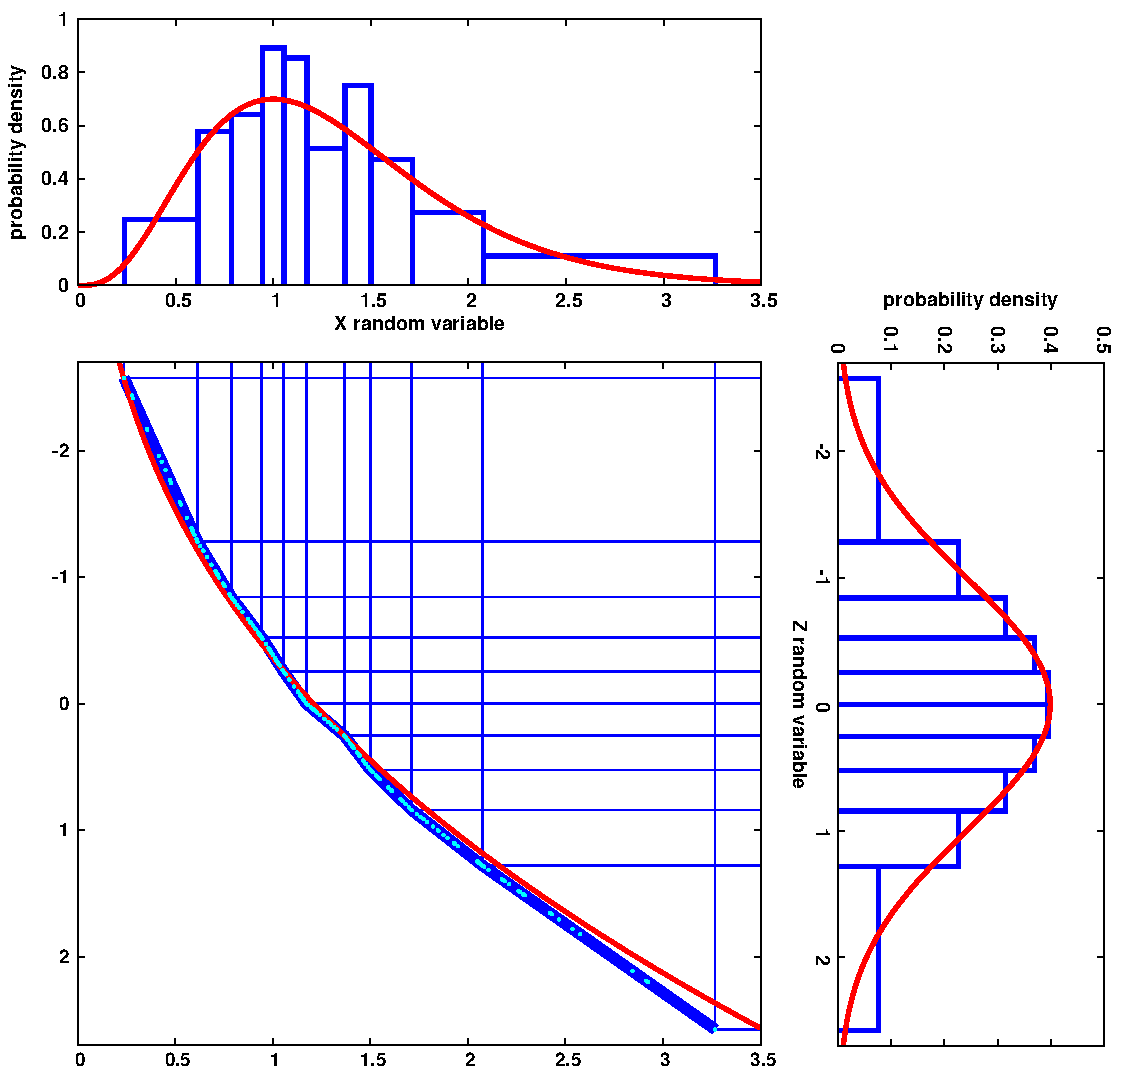
\includegraphics[width=0.685\textwidth]{Figures/ensanam_general_scheme.pdf}
}
\caption{Approximate piecewise linear anamorphosis transformation
(thick blue curve), remapping the deciles~$\tilde{x}_k$
of a 200-member random sample of the Gamma distribution $\Gamma(k,\theta)$
(top histogram) on the Gaussian deciles~$\tilde{z}_k$ (left histogram),
as compared to the exact transformation (in red) transforming the exact
$\Gamma(k,\theta)$ (red curve superposed to the top histogram)
into ${\cal N}(0,1)$ (red curve superposed to the left histogram).
\label{fig:anascheme}}
\end{figure*}

Figure~\ref{fig:anascheme} illustrates the behaviour of the algorithm by the transformation
of a gamma distribution into a Gaussian distribution, using a 200-member ensemble.
The application of the piecewise linear transformation (in blue in the figure)
can be performed using the module {\tt\bf anatra}
(using the ensemble quantiles provided by {\tt\bf anaqua}).

\subsection{Discrete events}
\label{sec:discrete}

In many practical applications, there can be problems in which a finite probability
concentrates on some critical value~$x_c$ of the state variable.
In this case the cdf~$F(x)$ is discontinuous and the standard anamorphosis transformation
described by Eq.~(\ref{eq:anaforward}) does not apply.

\begin{figure*}[htbp]
\centerline{
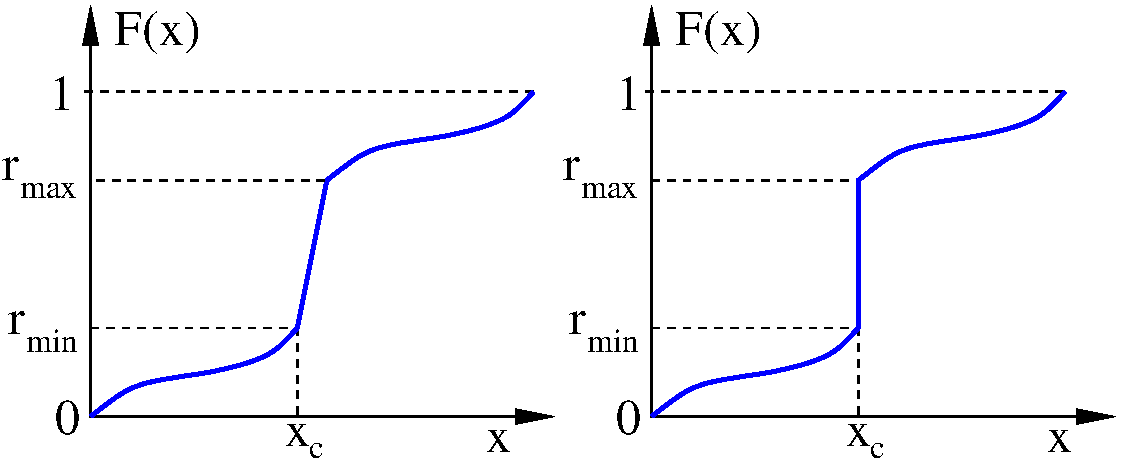
\includegraphics[width=0.685\textwidth]{Figures/ensanam_discrete_event.pdf}
}
\caption{As long as there is a slope in the cdf (left panel),
we know which value of the rank $r=F(x)$ corresponds to every value of~$x$.
As soon as the slope becomes a step at~$x_c$ (right panel),
we do not know anymore which rank~$r$, between $r_{\min}$ and~$r_{\max}$,
should correspond to~$x_c$.
\label{fig:anadiscrete}}
\end{figure*}

To generalize the algorithm, we can imagine the discontinuity in~$F(x)$
as the limit of a very steep slope (as illustrated in figure~\ref{fig:anadiscrete}).
As long as there is a slope (left panel), we know which value of the rank $r=F(x)$
corresponds to every value of~$x$: a small uncertainty in~$x$ just produces
a larger uncertainty in~$r$ when the slope is steeper.
As soon as the slope becomes a step (right panel),
we do not know anymore which rank~$r$, between $r_{\min}$ and~$r_{\max}$,
should correspond to~$x_c$.

The solution is then to make the transformation stochastic and transform~$x$
to a random rank (with uniform distribution) between $r_{\min}$ and~$r_{\max}$.
In this way, the forward transformation will transform the marginal distribution
of all variables to the target distribution [with cdf $G(z)$] as required,
the discrete events being transformed into a continuous variable
by the stochastic transformation; and the backward transformation
will transform it back to a discrete event, by transforming all ranks
between $r_{\min}$ and~$r_{\max}$ to~$x_c$.

\subsection{Extreme events}
\label{sec:extreme}

With an ensemble of size~$m$, there is a probability~$\frac{1}{m+1}$
that the value of any variable~$x$ is above tha maximum of the ensemble,
and the same probability that it is below the minimum.
These extreme events are missed by the ensemble,
so that the tails of the marginal distributions cannot be transformed
into Gaussian tails using the method described above
(which is based on the available ensemble only).
If dealing adequately with extreme events
(outside the range of the ensemble) is important,
an additional source of information is needed.

One possible solution to this problem is to have a wider catalogue
of possible realization of~$x$
(like climatological data, historical records or data from nearby space/time location,
by assuming space or time homogeneity of the statistics),
and use this catalogue to specify the shape of the tails of the probability distributions.
For instance, the quantiles of the ensemble can be merged with the quantiles of the catalogue
to obtain an extended description of the transformation function.
This simple solution is implemented in the module {\tt\bf anatail}.

\subsection{Transformation of observations}
\label{method:obs}

In many practical situations, if the observation operator~${\cal H}$ is simple enough,
it may be equivalent%
\footnote{It is equaivalent if ${\cal H}$ is linear or if the observational
update is performed using a linear scheme.}
or sufficient to describe the dependence between ${\bf x}$ and~${\bf y} = {\cal H}({\bf x})$
using the statistics of the prior ensemble.
Following this assumption, we can then augment the state vector with~${\bf y}$:

$${\bf X} = \left[ \begin{array}{l} {\bf x} \\ {\bf y} = {\cal H}({\bf x}) \end{array} \right]$$

\noindent
and consider ${\bf y}^o$ as direct observation of the component~${\bf y}$ of~${\bf X}$.
Anamorphosis transformation functions are then computed for all variables of~${\bf X}$
including the equivalent of each observation $y^o_j$ in~${\bf y}^o$.

If then, as a second assumption, the observation errors associated to every individual
observations~$y^o_j$ are assumed independent,
it becomes possible to transform the univariate distributions~$p(y^o_j|y_j)$
to a counterpart written in terms of the transformed variable~$A(y_j)$.
The benefit of this transformation of the observation error probability distribution
is to avoid including the backward transformation~$A_j^{-1}$ in the observation operator,
which would for instance be impossible in the context of a linear observational update algorithm
(since the $A_j^{-1}$ are nonlinear by construction).

To transform~$p(y^o_j|y_j)$, one possible solution is to draw a sample
of the possible ranks $r_{js},\,s=1,\ldots,N$ of observation~$y^o_j$
in the prior ensemble (adequately perturbed by observation error),
so that $G^{-1}(r_{js}$ provides a sample of the required transformed distribution.
For each draw of the sample $s=1,\ldots,N$, we need first to select
one possible rank~$r^o_s$ for the observation error.
Second, we perturb the observation equivalent of every member of the ensemble
with this observation error $\tilde{y}_j^i = F^{-1}_i(r_s^o)$,
where $F_i$ is the cdf of~$p(y|Hx_i)$ and $i$ is the index of the ensemble member.
And third, we compute the rank~$r_{js}$ of the observation~$y^o_j$
in the perturbed ensemble~$\tilde{y}_j^i$.
This algorithm can be rewritten using the anamorphic transformation
defined in section~\ref{sec:defana}, with the following steps:

\begin{itemize}
\item sample a rank for observation error $r^o_s$;
\item perturb the ensemble accordingly: $\tilde{y}_j ^i = F^{-1}_i(r_s^o)$;
\item compute anamorphic transformation~$A_s^o$ from this perturbed ensemble;
\item apply~$A_s^o$ to the observation: $A_s^o(y^o_j)$.
\end{itemize}

\noindent
By iterating this algorithm on~$s$, we obtain a sample of the transformed distribution.

If the probability distribution for observation errors~$p(\epsilon = y-Hx)$
is symmetric and independent of the state~$x$ of the system,
it is equivalent (and much less expensive) to perturb the observation~$y^o$
rather than the prior ensemble.
The algorithm simplifies to:

\begin{itemize}
\item perturb observation with observation error: $y^o_s = y^o + \epsilon_s$;
\item apply anamorphosis transformation to~$y^o_s$,
\end{itemize}

\noindent
where the anamorphosis transformation is computed using the observation equivalent
of the prior ensemble (without perturbation).

\section{Description of the modules}

In this section,
the modules are described one by one,
giving for each of them:
the method that has been implemented,
the list of public variables and public routines
(with a description of input and output data),
the MPI parallelization, and
an estimation of the computational cost
as a function of the size of the problem.

\subsection{Module: {\tt\bf anaqua}}

The purpose of this module is to compute the quantiles of the ensemble
defining the anamorphosis transformation functions.

\subsubsection*{Method}

The approach is to loop over all variables,
sort the ensemble for each variable (with the heap sort algorithm), and
compute the quantiles by linear interpolation in the sorted ensemble.
Options are provided to deal with ensemble members with unequal weights
(either a global weight or a different weight for every variable).
In this case, the interpolation to compute the quantiles
is based on the cumulated weights.

\subsubsection*{Public variables}

None.

\subsubsection*{Public routines}

\begin{description}
\item[ens\_quantiles:] to compute the quantiles of the ensemble:
  \begin{description}
  \item[{\tt qua} (output)]: quantiles of the ensemble;
  \item[{\tt ens} (input)]: ensemble;
  \item[{\tt quadef} (input)]: definition of the quantiles (list of the required ranks);
  \item[{\tt enswei} (input, optional)]: global weight for each ensemble member (default=equal weights);
  \item[{\tt ensweiloc} (input, optional)]: local weights for each ensemble member and each variable (default=equal weights).
  \end{description}
\end{description}

\subsubsection*{MPI parallelization}

For ensemble with many state variables,
MPI parallelization is easily obtained by making each processor
work on a different part of the state vector.
Since the operations on different state variables are independent,
no MPI operations needed to be implemented inside the routine.

\subsubsection*{Computational cost}

The computational complexity of the algorithm can be written:

\begin{equation}
C \sim k_1 n  m \log m + k_2 n
\end{equation}

\noindent
where $n$ is the number of state variables,
$m$, the size of the ensemble, and
$k_1,\,k_2$, are order~1 constants.
The first term corresponds to the sorting of the input ensemble,
and the second term to the interpolation in the sorted ensemble.

\subsection{Module: {\tt\bf anatra}}

The purpose of this module is to apply forward and backward
anamorphosis transformation functions.

\subsubsection*{Method}

The approach is to loop over all variables,
localize the variable to transform among the ensemble quantiles, and
linearly interpolate among the corresponding quantiles of the target distribution.
The transformation deals with discrete events (non-distinct quantiles)
using random transformation in the range of the corresponding quantiles.

\subsubsection*{Public variables}

None.

\subsubsection*{Public routines}

\begin{description}
\item[ana\_forward:] forward anamorphosis transformation of input ensemble/vector/variable:
  \begin{description}
  \item[{\tt ens/vct/var} (input/output)]: ensemble/vector/variable to transform;
  \item[{\tt qua} (input)]: ensemble quantiles (provided by module {\tt\bf anaqua});
  \item[{\tt quaref} (input)]: quantiles of the target distribution;
  \item[{\tt rank} (input, optional)]: rank to use for discrete event (default=random).
  \end{description}
\item[ana\_backward:] backward anamorphosis transformation of input ensemble/vector/variable:
  \begin{description}
  \item[{\tt ens/vct/var} (input/output)]: ensemble/vector/variable to transform;
  \item[{\tt qua} (input)]: ensemble quantiles (provided by module {\tt\bf anaqua});
  \item[{\tt quaref} (input)]: quantiles of the target distribution.
  \end{description}
\end{description}

\subsubsection*{MPI parallelization}

For ensemble with many state variables,
MPI parallelization is easily obtained by making each processor
work on a different part of the state vector.
Since the operations on different state variables are independent,
no MPI operations needed to be implemented inside the routine.

\subsubsection*{Computational cost}

The computational complexity of the algorithm can be written:

\begin{equation}
C \sim k_1 n  \log q + k_2 n
\end{equation}

\noindent
where $n$ is the number of variables to transform,
$q$, the number of quantiles used to define the transformation, and
$k_1,\,k_2$, are order~1 constants.
The first term corresponds to the localization of the variable in the list of quantiles,
and the second term to the interpolation between the quantiles.

\subsection{Module: {\tt\bf anaobs}}

The purpose of this module is to apply forward
anamorphosis transformation to the observation
error probability distribution.

\subsubsection*{Method}

In the general case, the approach is to loop over all variables,
perturb the ensemble according to observation error probability distribution
(with the same rank for all members),
compute the quantiles of this perturbed ensemble,
and use these quantiles to transform the input observation.
This operation is then repeated several times
to produce a sample of the transformed observation error probability distribution.

In case of a symmetric observation error probability distribution,
the approach is to loop over all variables,
apply perturbation to the input observation,
and apply forward anamorphosis using the quantiles of the ensemble.
This operation is then repeated several times
to produce a sample of the transformed observation error probability distribution.

\subsubsection*{Public variables}

None. The type of observation error probability distribution
(`gaussian', `lognormal', `gamma' or `beta', default=`gaussian')
is defined through the module {\bf\tt obserror}.

\subsubsection*{Public routines}

\begin{description}
\item[ana\_obs:] transformation of observation error probability distribution (general case):
  \begin{description}
  \item[{\tt anaobs} (output)]: sample of transformed observation error probability distribution;
  \item[{\tt obsens} (input)]: ensemble equivalent to observations;
  \item[{\tt obs} (input)]: observation vector to be transformed;
  \item[{\tt obserror} (input)]: spread of observation error (precise meaning depending on the type of distribution);
  \item[{\tt quadef} (input)]: definition of the quantiles used for anamorphosis;
  \item[{\tt quaref} (input)]: quantiles of the target distribution.
  \end{description}
\item[ana\_obs\_sym:] transformation of observation error probability distribution (symmetric case):
  \begin{description}
  \item[{\tt anaobs} (output)]: sample of transformed observation error probability distribution;
  \item[{\tt obs} (input)]: observation vector to be transformed;
  \item[{\tt obserror} (input)]: spread of observation error (precise meaning depending on the type of distribution);
  \item[{\tt obsqua} (input)]: quantiles of ensemble equivalents to observations (provided by module {\tt\bf anaqua});
  \item[{\tt quaref} (input)]: quantiles of the target distribution.
  \end{description}
\end{description}

\subsubsection*{MPI parallelization}

For problems with many observations,
MPI parallelization is easily obtained by making each processor
work on a different part of the observation vector.
Since the operations on different observations are independent,
no MPI operations needed to be implemented inside the routine.

\subsubsection*{Computational cost}

In the general case, the computational complexity of the algorithm can be written:

\begin{equation}
C \sim k_1 n s m  +  k_2 n s m \log m + k_3 n s ( k_4 + \log q )
\end{equation}

\noindent
where $n$ is the number of variables to transform,
$m$, the size of the ensemble,
$s$, the size of the sample to produce,
$q$, the number of quantiles used to define the transformation,
$k_1$, the cost of sampling the univariate observation error probability distribution, and
$k_2,\,k_3\,k_4$, are order~1 constants.
The first term corresponds to the perturbation of the ensemble,
the second term to the computation of the quantiles of the perturbed ensembles,
and the third term to the transformation of the observation vector.

In case of a symmetric observation error probability distribution,
this cost is reduced to:

\begin{equation}
C \sim k_1 n s + k_3 n s ( k_4 + \log q )
\end{equation}

\noindent
The first term corresponds to the perturbations of the observation vector,
and the second term to the transformation of the perturbed observation vectors.

\subsection{Module: {\tt\bf anatail}}

Module not yet available.

\begin{thebibliography}{}

\bibitem[Brankart et al.(2012)]{BRAN12}
Brankart, J.-M., C.-E. Testut, D.~B\'eal, M.~Doron, C.~Fontana, M.~Meinvielle,
P.~Brasseur, and J.~Verron, 2012: Towards an improved description of ocean
uncertainties: effect of local anamorphic transformations on spatial
correlations. \textit{Ocean Science}, \textbf{8}, 121--142.

\end{thebibliography}


\end{document}

